\chapter{Billiard-AI}
In diesem Kapitel werden die gewählte Architektur wie auch die bisher erarbeiteten theoretischen Ansätze behandelt.
Weiterhin wird auf verschiedene Aspekte des Aufbaus und dessen Problematik eingegangen.

\section{Aufbau und Messung}\label{kap:aufbauMessung}
Die Kamera wie auch der Projektor werden mittels eines Baugerüsts über dem Tisch platziert. Dieses ermöglicht die nötige
Flexibilität, um die optischen Objekte unabhängig voneinander optimal auszurichten.
TODO: Bild einfügen

Der Tisch ist an den Seiten leicht schräg, was ein genaues Messergebnis verunmöglicht. Weiterhin ist er an den Kanten
nicht fest und kann leicht deformiert werden. Um diese Ungenauigkeitsfaktoren möglichst gering zu halten, wurden die
gegenüberliegenden Tischkanten mit je zwei Holzstücken (Abbildung \ref{fig:messung:tisch}, 1), deren Breite individuell
über einen Messschieber millimetergenau bestimmt wurde, ausgestattet. Nun kann die Distanz zwischen den Holzstücken
gemessen und anschliessend die Breite der Hölzer dazuaddiert werden. Die Messung selbst (Abbildung \ref{fig:messung:tisch}, 2 und 3)
wird über ein Laser-Messgerät\footnote{Die genauen Spezifikationen sind im Anhang \ref{anhang:messung:messgeraete} ersichtlich.}
durchgeführt. Die Messungenauigkeit wird mit $\pm 1.5mm$ angegeben. Die Abbildung \ref{fig:messung:tisch} zeigt die Messung in X-Richtung,
diese Messung wird ebenfalls in gleicher Art und Weise in Y-Richtung durchgeführt.
\begin{figure}[h!]
    \begin{center}
        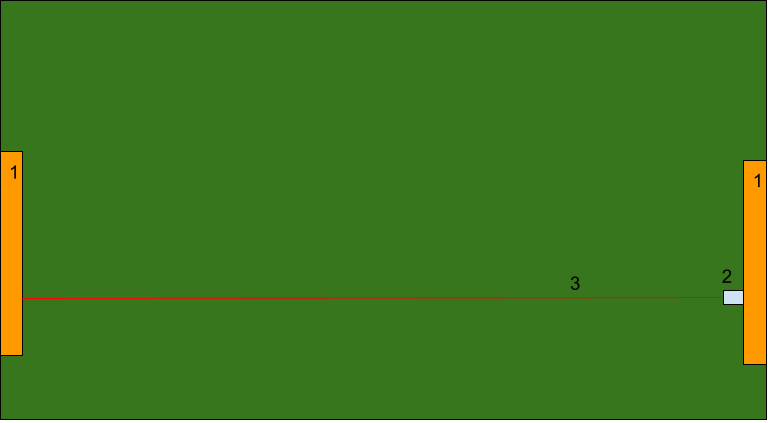
\includegraphics[width=0.8\linewidth]{../common/03_billiard_ai/resources/01_messung_tisch.png}
    \end{center}
    \caption{Messung - Tisch}
    \label{fig:messung:tisch}
\end{figure}


Um die Messung der Kugeln zu erläutern, muss zuerst das Koordinatensystem eingeführt werden. Die Kugeln selbst werden
über eine Kamera aufgenommen und deren Position daher auch in einem Pixelkoordinatensystem bestimmt. Dies ist aus
mehreren Gründen ungünstig. Einerseits soll die allgemeine Abhängigkeit zur Kamera vermieden werden, andererseits ist das
Pixelkoordinatensystem für die Visualisierung nicht gut geeignet.\\
Die Kugeln werden also in ein Modellkoordinatensystem übersetzt\footnote{Siehe Kapitel \ref{kap:koordinatenUmrechnung}}.
Bei diesem befindet sich der Ursprung in der Mitte des Tisches und die X- wie auch die Y-Achse bilden die Breite und Höhe
in Millimeter ab.

Um nun die Position der Kugel zu bestimmen, wird zuerst deren Abstand zu den Banden gemessen (siehe Abbildung \label{fig:messung:kugel}, 1 und 2).
Dies geschieht wie beim Ausmessen des Tisches über ein Holzstück und das Lasermessgerät. Wurden beide Distanzen bestimmt, so
kann der Mittelpunkt der Kugel berechnet werden, indem noch der Radius, welcher durch einen Messschieber bestimmt wurde, dazuaddiert wird.
Es gilt nun, diesen Punkt in das Modellkoordinatensystem zu übersetzen. Dazu wird jeweils die halbe Breite wie auch Höhe
(beachte den Ursprung des Modellkoordinatensystems) von dem Mittelpunkt abgezogen. Abschliessend werden noch die korrekten
Vorzeichen über den Quadranten bestimmt.

\begin{figure}[h!]
    \begin{center}
        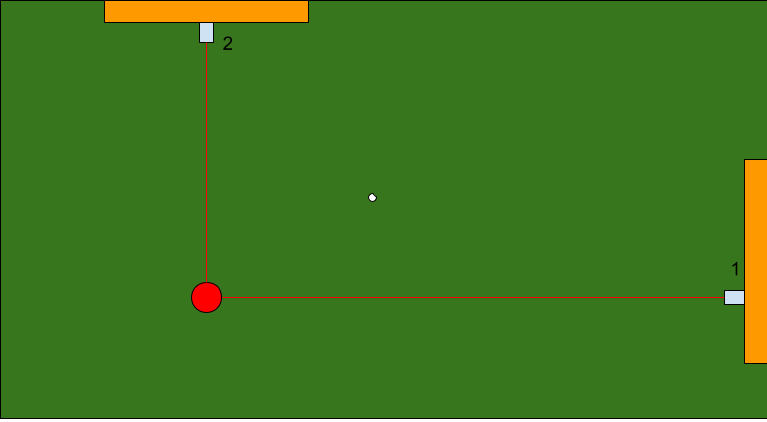
\includegraphics[width=0.8\linewidth]{../common/03_billiard_ai/resources/02_messung_kugel.png}
    \end{center}
    \caption{Messung - Kugel}
    \label{fig:messung:kugel}
\end{figure}

\section{Architektur}
Die eigentliche Funktionalität wird in einer Core-Library untergebracht, welche nativ in C++ entwickelt wird. Das
Endprodukt soll aber weitaus mehr zu bieten haben, wie aus den Zielen ersichtlich wird. Deswegen wird in Unity eine
Interaktionsmöglichkeit geschaffen, worüber der Benutzer einerseits die Resultate visualisiert erhält und
andererseits der Core-Library seine nächsten Schritte mitteilen kann. Um dies zu erreichen, wird eine weitere native
Komponente erstellt, welche die Interaktion zwischen Unity und der Core-Library ermöglicht. Es ist dies eine C/C++-Bibliothek,
die ein C-Interface bereitstellt, welches in Unity geladen wird. Unity selbst erhält ebenfalls eine Abstraktionsschicht,
um die Nativen auf die Applikationsmodelle zu mappen. Eine Darstellung kann in Abbildung \ref{fig:top-level-architecture} entnommen
werden.

\begin{figure}[h!]
    \begin{center}
        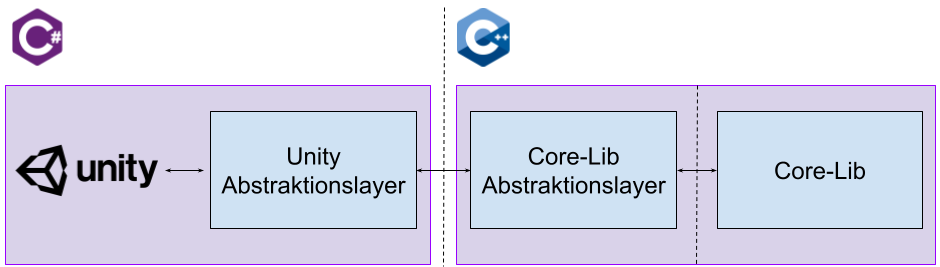
\includegraphics[width=0.8\linewidth]{../common/03_billiard_ai/resources/00_top_level_architecture.png}
    \end{center}
    \caption{Grobarchitektur - Applikationsumgebung}
    \label{fig:top-level-architecture}
\end{figure}

Die Core-Library selbst besteht aus mehreren Teilstücken. Es sind dies namentlich mitsamt Funktionalität die
folgenden:
\begin{description}
    \item[billiard\textunderscore capture] Erfasst den aktuellen Spielstand und stellt diesen im OpenCV-Format bereit.
    \item[billiard\textunderscore detection] Erstellt aus dem Spielstand eine interne Repräsentation, welchen den Status beschreibt.
    \item[billiard\textunderscore search] Verwendet den aktuellen Status wie auch eine zusätzliche Such-Beschreibung, um einen optimalen
    Stoss zu berechnen.
    \item[billiard\textunderscore physics] Stellt Funktionalität bereit, um physikalische Berechnungen durchzuführen.
\end{description}

\section{Von Pixel zu Modellkoordinaten}\label{kap:koordinatenUmrechnung}
TODO: Write ArUco